
\subsection{Rezultati testiranja stranice pojedinog blog posta}
\label{sec:rezultati-blog-post}

\begin{figure}[H]
    \centering
    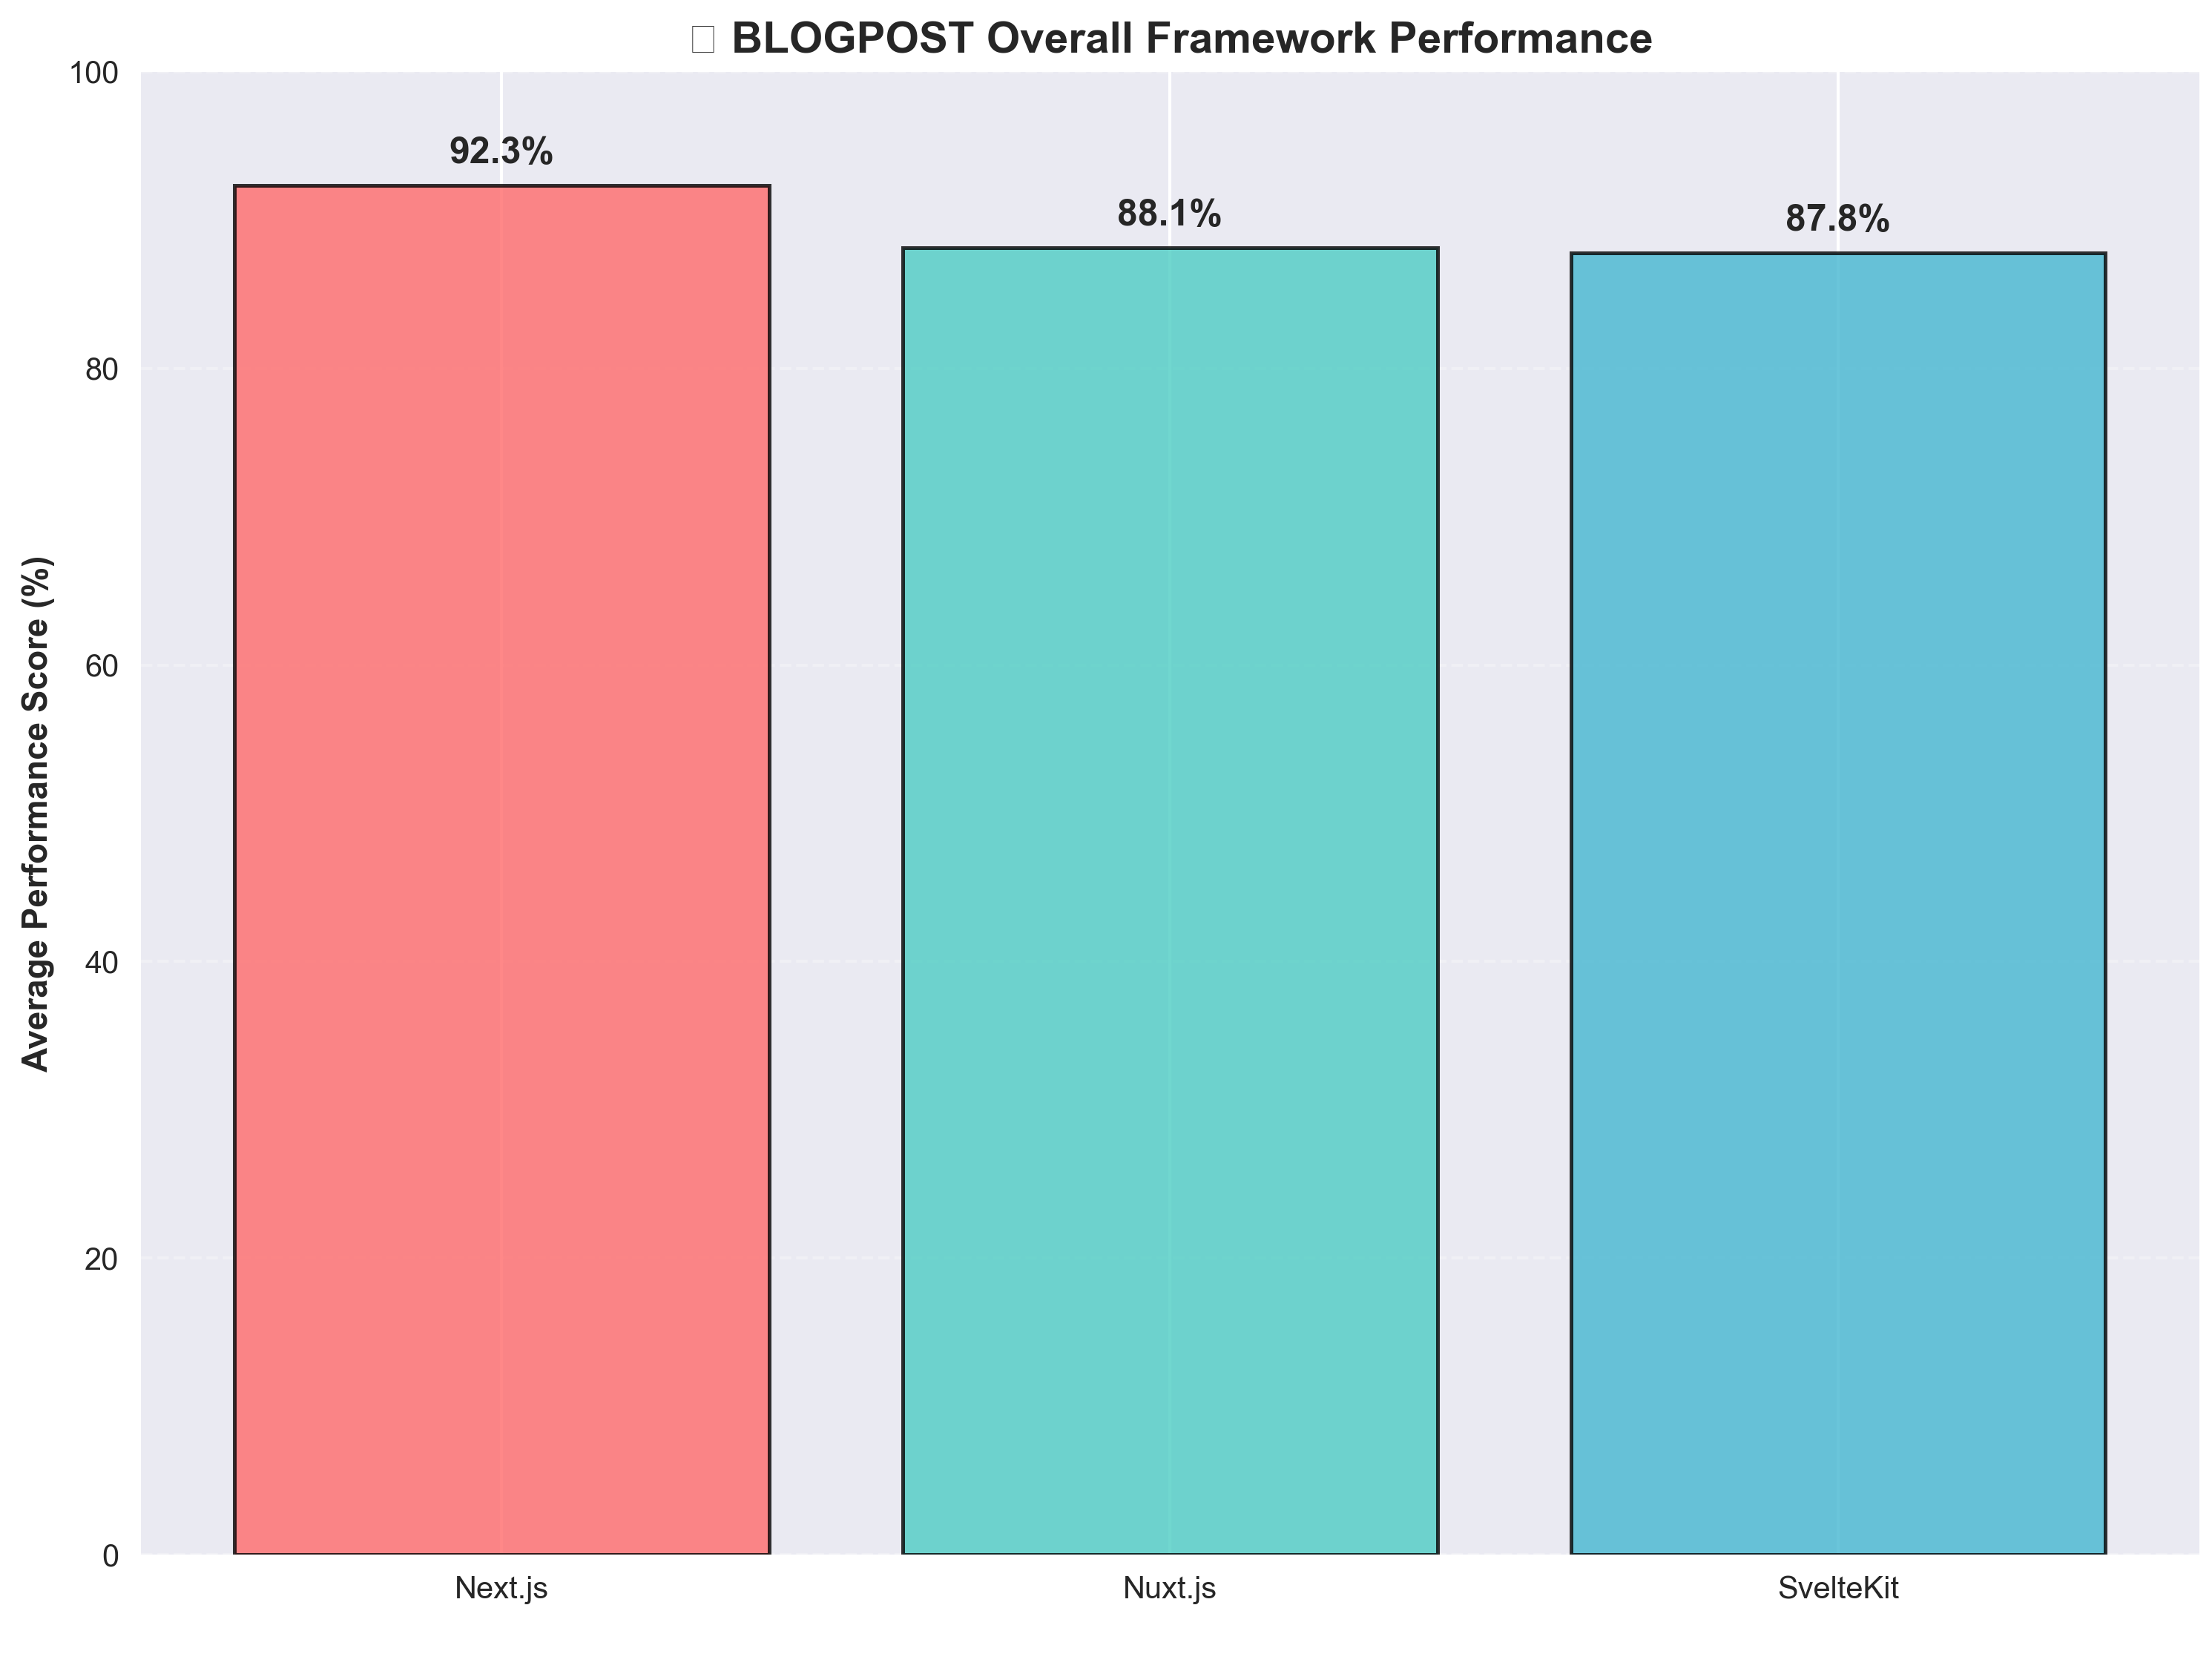
\includegraphics[width=0.8\textwidth]{slike/rezultati/blog-post/blogPost_framework_overall_performance.png}
    \caption{Ukupne ocjene radnih značajki (stranica pojedinog bloga) }
    \label{fig:testiranje-blog-post-ukupne-performanse}
\end{figure}

\begin{figure}[H]
    \centering
    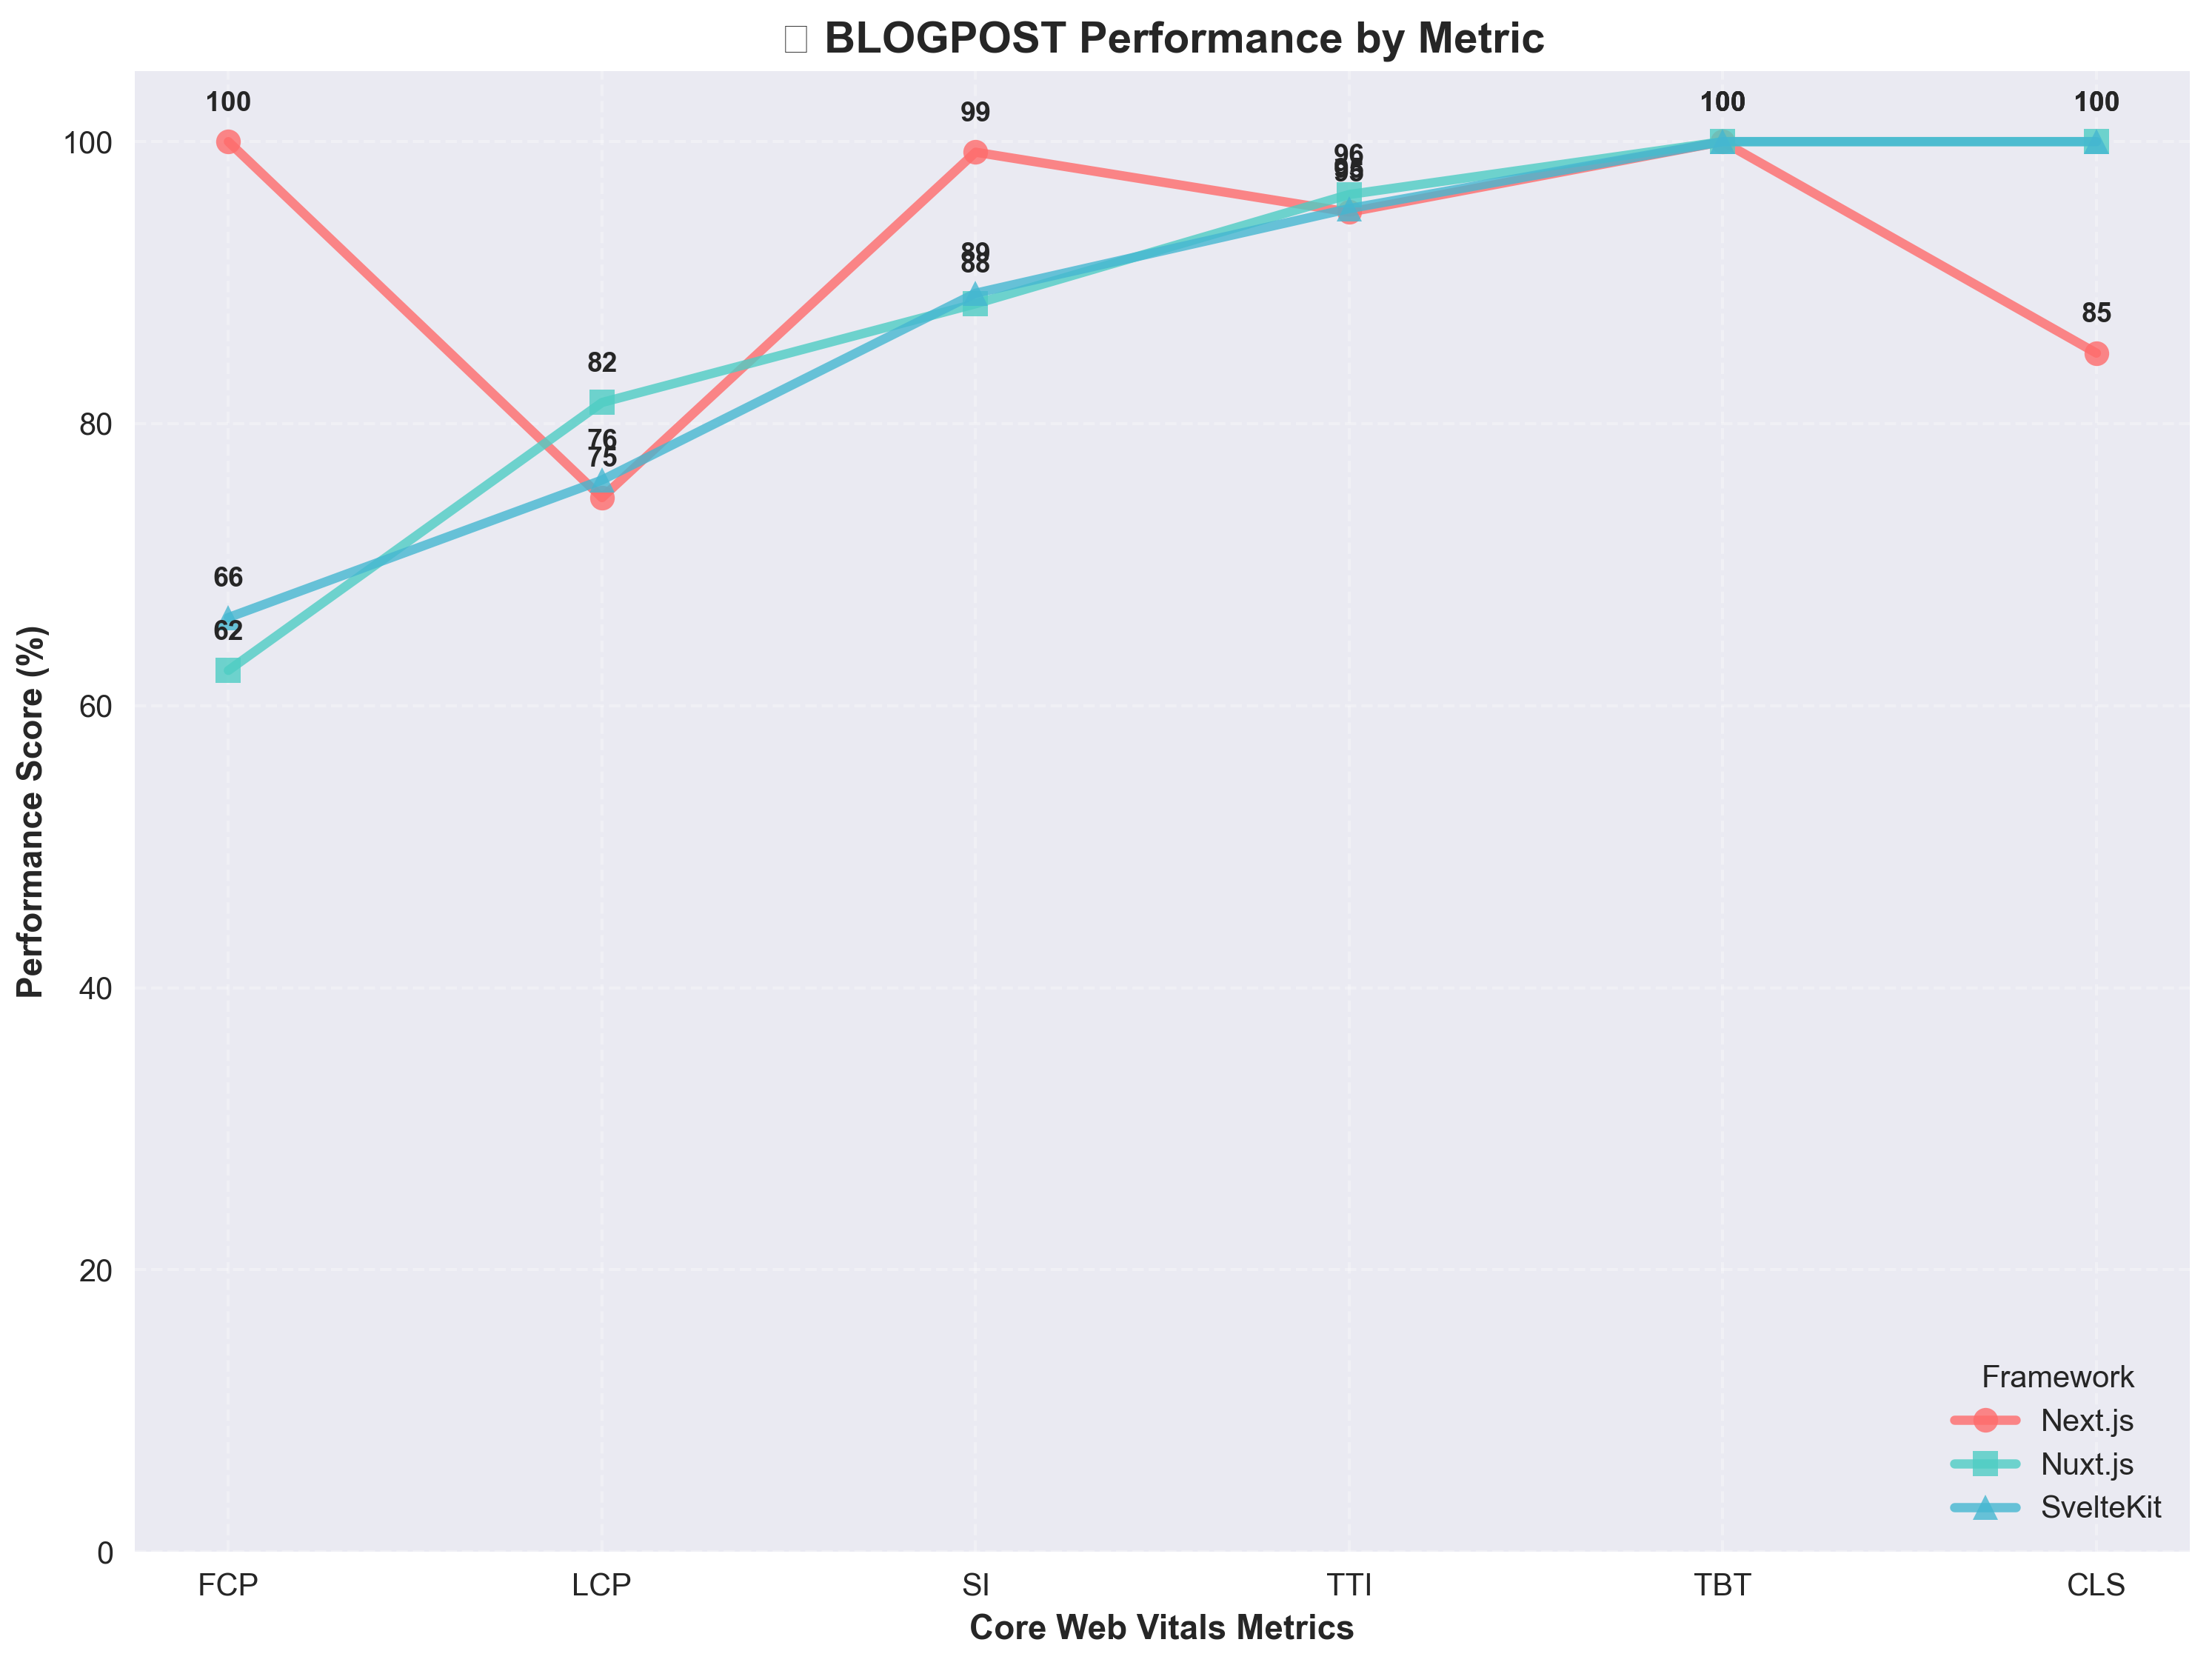
\includegraphics[width=0.8\textwidth]{slike/rezultati/blog-post/blogPost_performance_by_metric.png}
    \caption{Ukupne ocjene radnih značajki po metrici (stranica pojedinog bloga) }
    \label{fig:testiranje-blog-post-performanse-po-metrici}
\end{figure}

\begin{figure}[H]
    \centering
    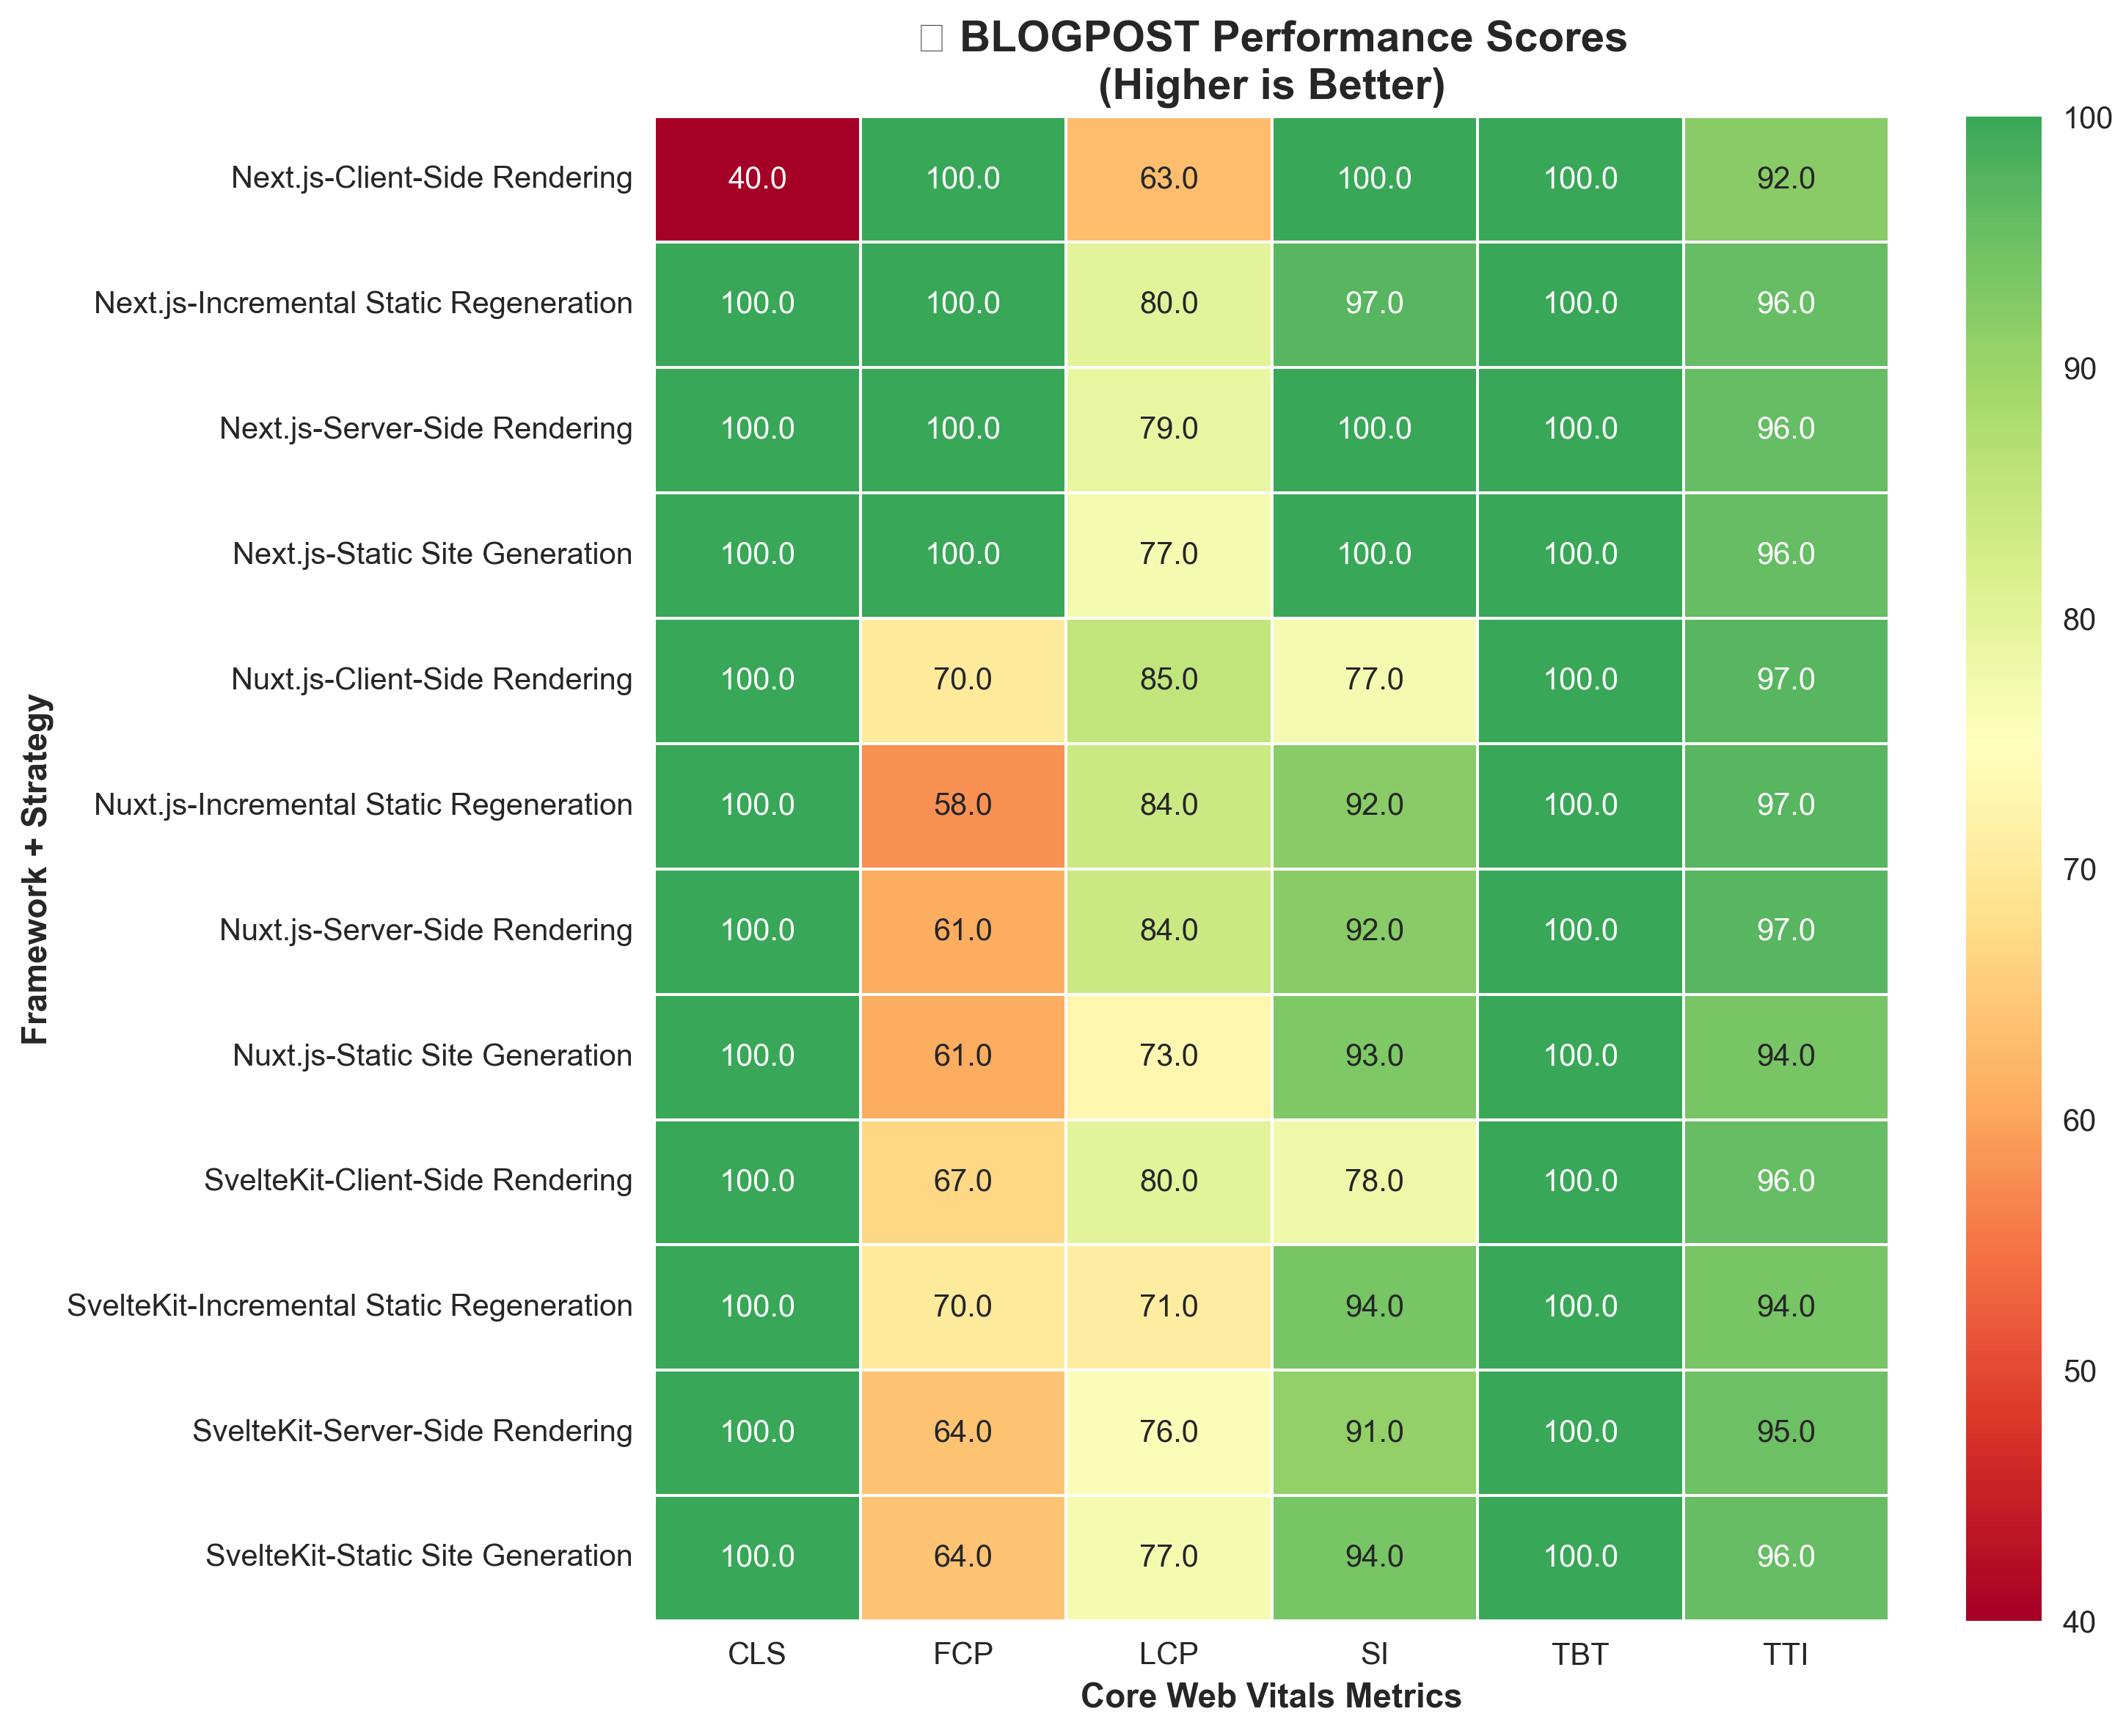
\includegraphics[width=\textwidth]{slike/rezultati/blog-post/blogPost_performance_scores.png}
    \caption{Ocjene radnih značajki - postotak (stranica pojedinog bloga) }
    \label{fig:testiranje-blog-post-postotak}
\end{figure}

\begin{figure}[H]
    \centering
    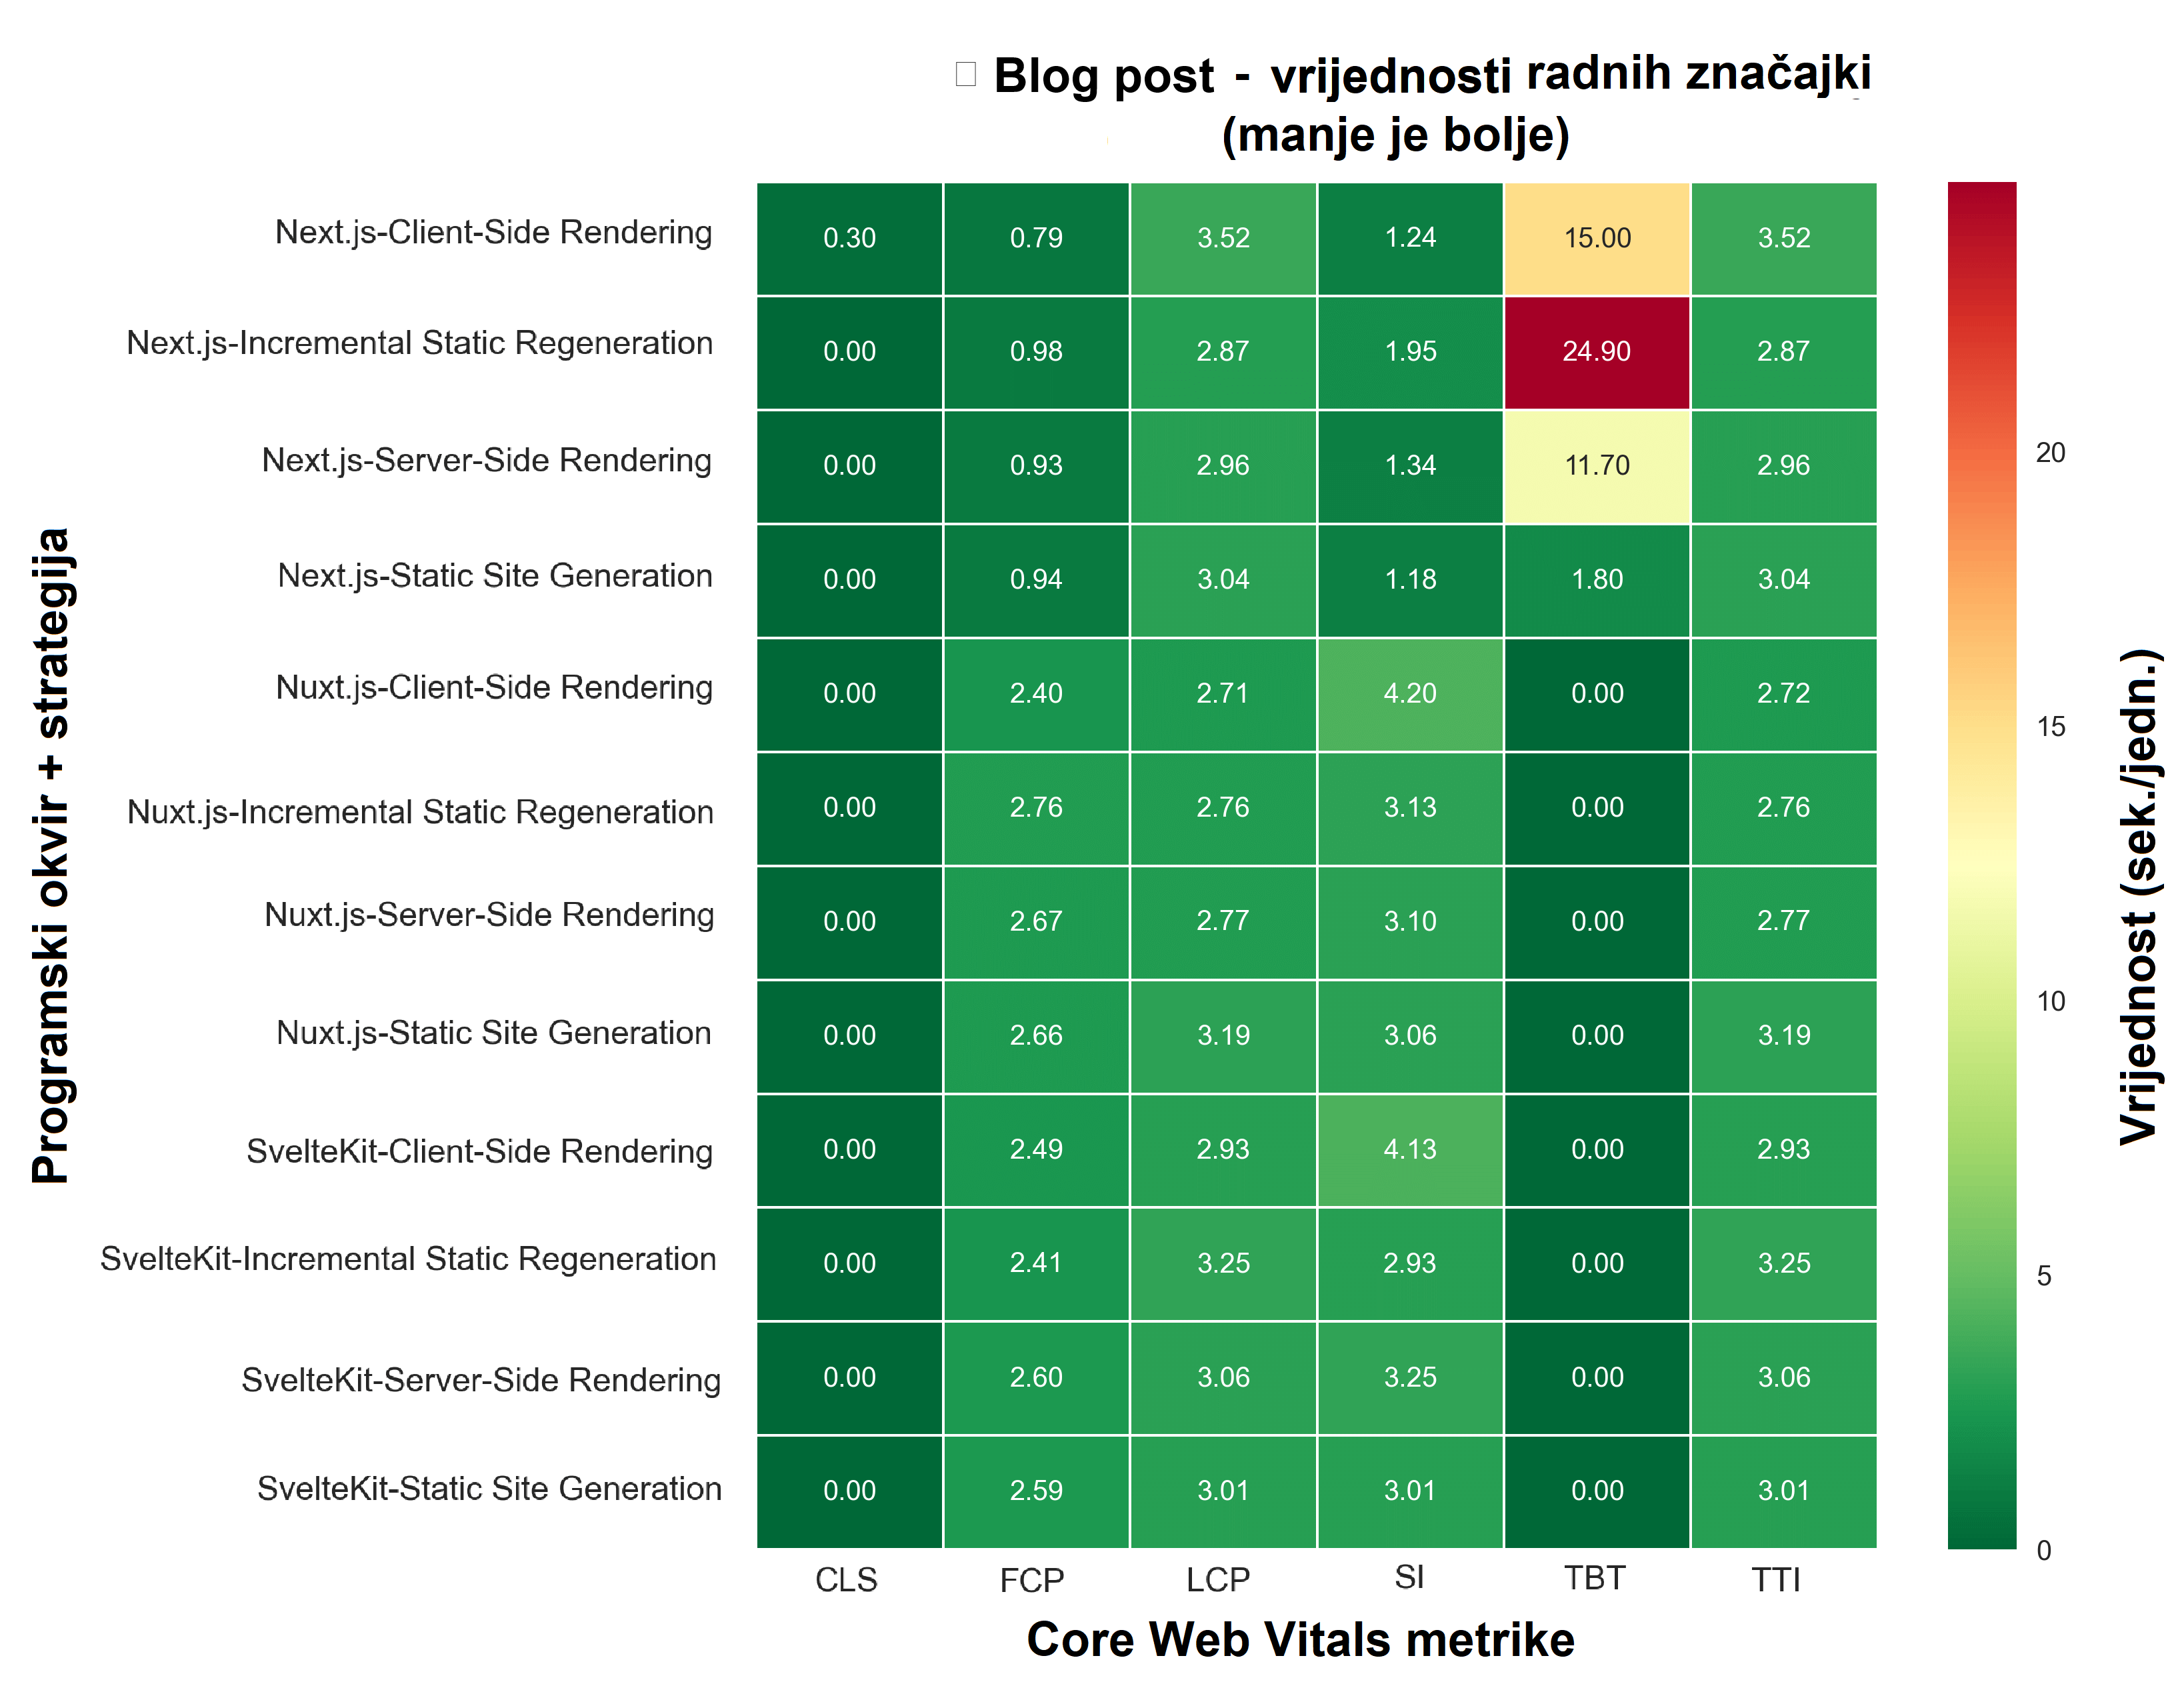
\includegraphics[width=\textwidth]{slike/rezultati/blog-post/blogPost_performance_values.png}
    \caption{Ocjene radnih značajki - vrijednosti (stranica pojedinog bloga) }
    \label{fig:testiranje-blog-post-vrijednosti}
\end{figure}

\begin{figure}[H]
    \centering
    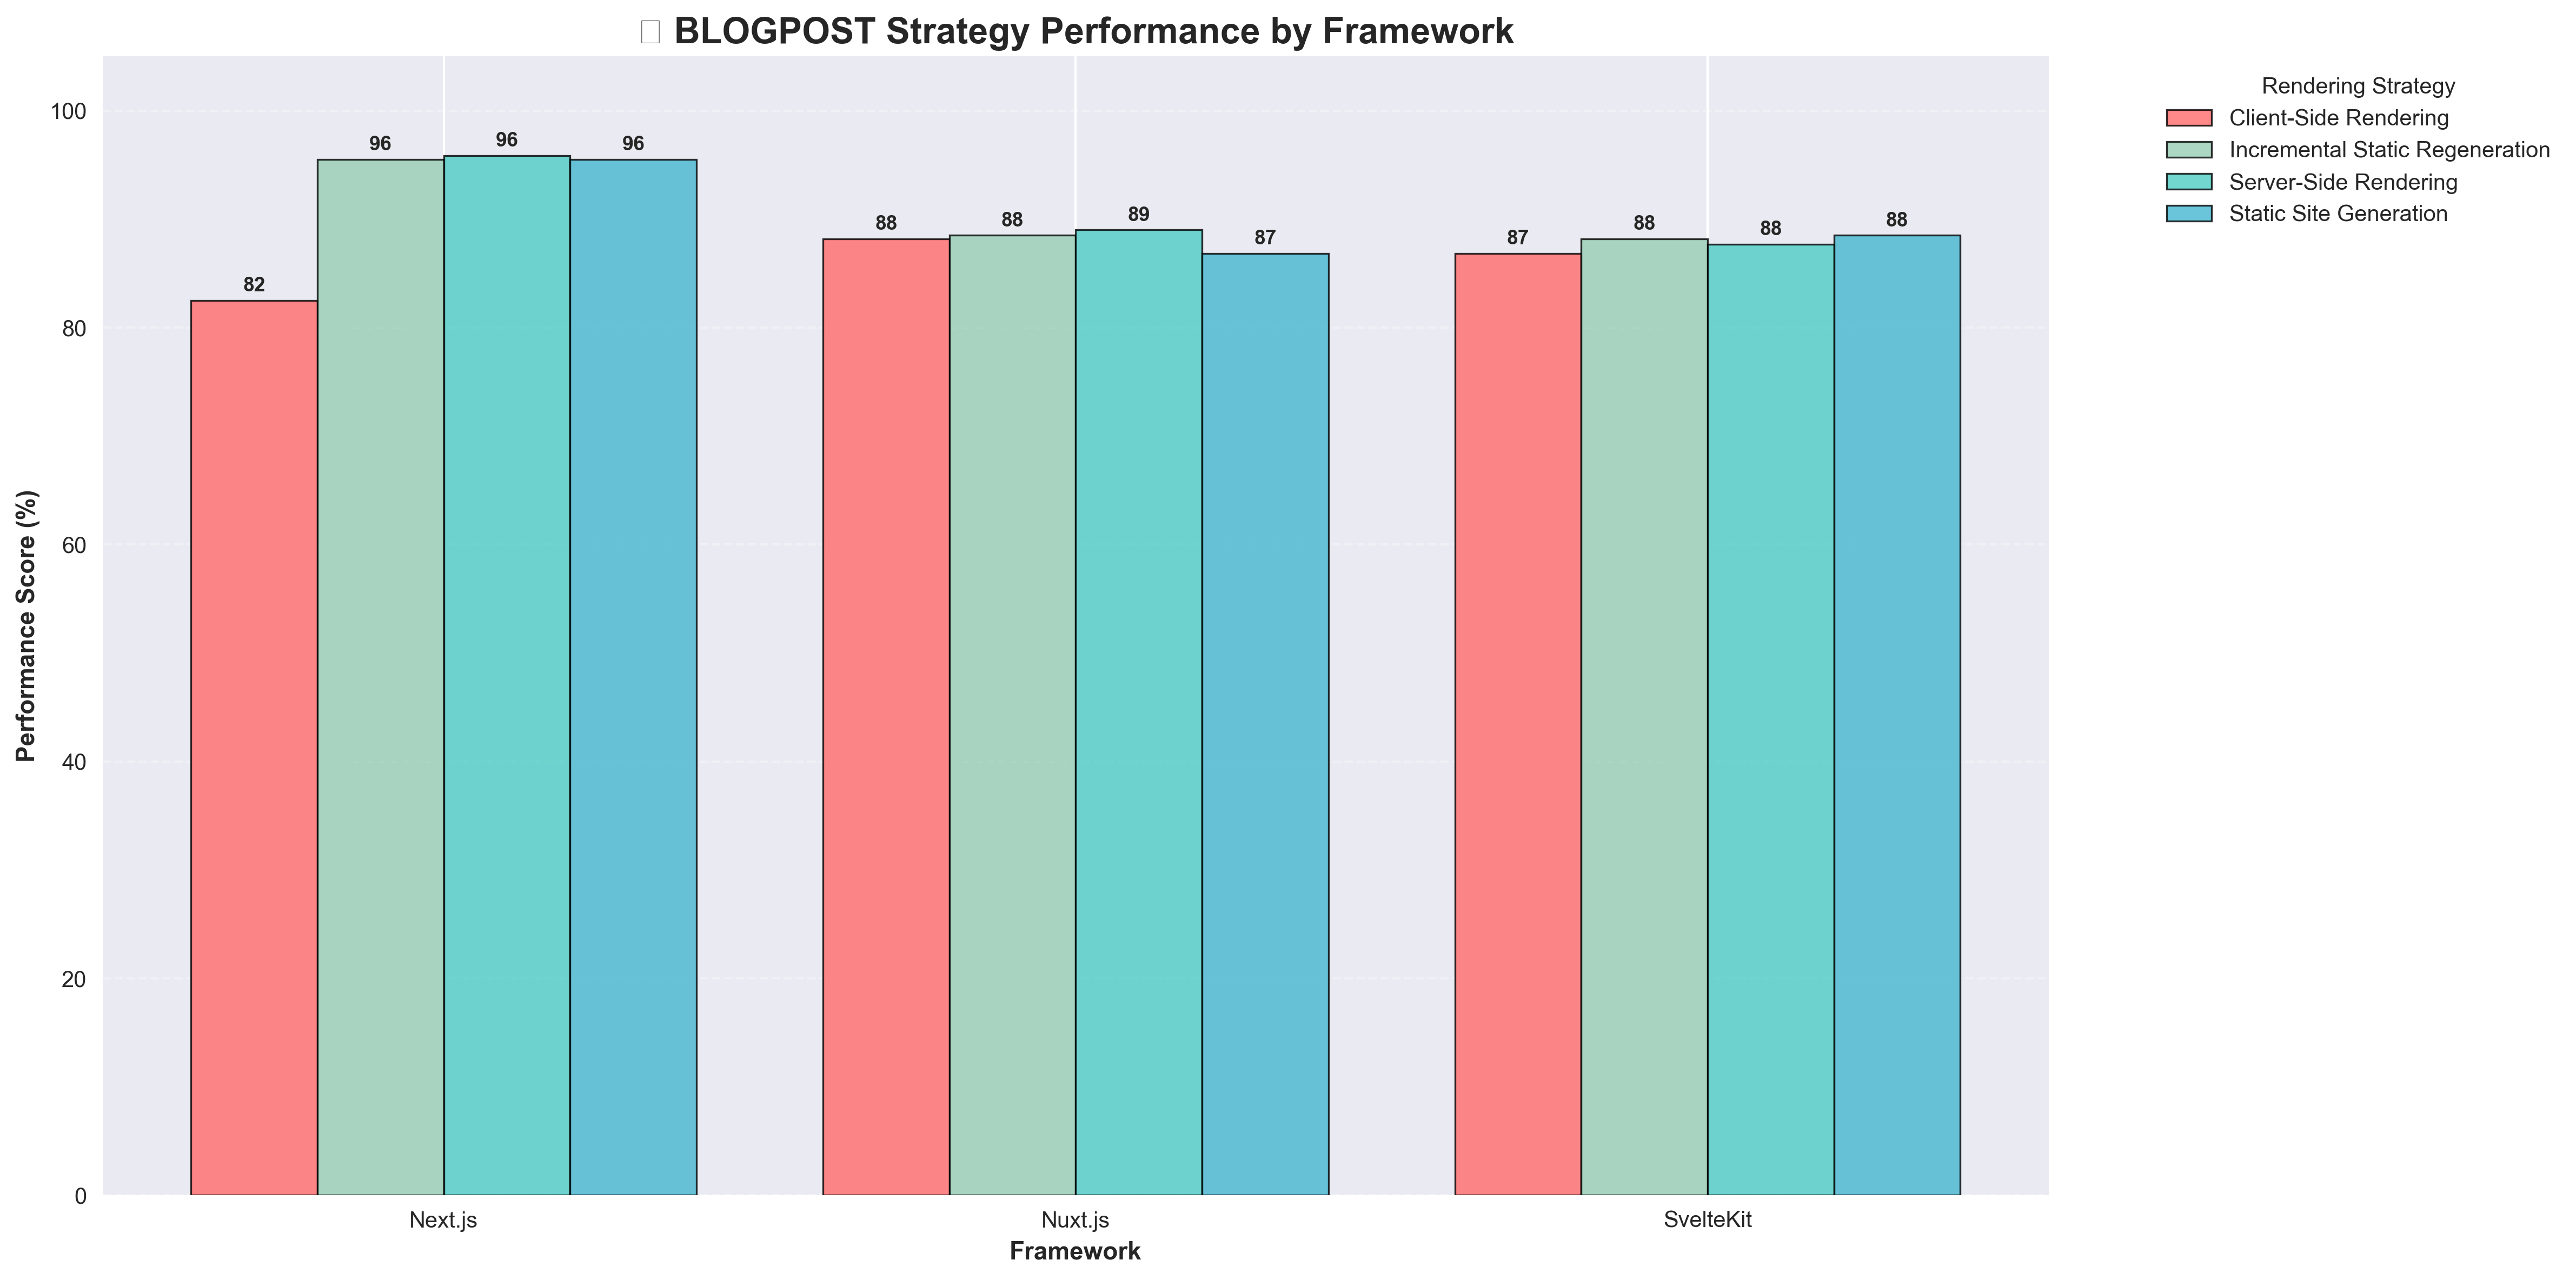
\includegraphics[width=\textwidth]{slike/rezultati/blog-post/blogPost_strategy_comparison.png}
    \caption{Ocjene radnih značajki - usporedba strategija (stranica pojedinog bloga) }
    \label{fig:testiranje-blog-post-usporedba-strategija}
\end{figure}

\newpage

\subsection{Sažetak rezultata - stranica pojedinog blog posta}

\begin{table}[H]
    \centering
    \caption{Sažetak rezultata testiranja stranice pojedinog bloga}
    \label{tab:sazetak-rezultata-blog-post}
    \renewcommand{\arraystretch}{1.5}
    \resizebox{\textwidth}{!}{%
        \begin{tabular}{|l|l|l|}
            \hline
            \textbf{Kategorija} & \textbf{Element}                             & \textbf{Ocjena}    \\
            \hline
            \multirow{3}{*}{\textbf{Programski okviri}}
                                & 1. Next.js                                   & 92.3\% (±14.8\%)  \\[0.2em]
                                & 2. Nuxt.js                                   & 88.1\% (±14.1\%)  \\[0.2em]
                                & 3. SvelteKit                                 & 87.8\% (±13.3\%)  \\
            \hline
            \multirow{4}{*}{\textbf{Strategije iscrtavanja}}
                                & 1. Server-Side Rendering                     & 90.8\% (±12.8\%)  \\[0.2em]
                                & 2. Incremental Static Regeneration           & 90.7\% (±12.8\%)  \\[0.2em]
                                & 3. Static Site Generation                    & 90.3\% (±13.4\%)  \\[0.2em]
                                & 4. Client-Side Rendering                     & 85.8\% (±17.3\%)  \\
            \hline
            \multirow{5}{*}{\textbf{Najbolje kombinacije}}
                                & 1. Next.js + Server-Side Rendering           & 95.8\% (±8.4\%)   \\[0.2em]
                                & 2. Next.js + Incremental Static Regeneration & 95.5\% (±7.8\%)   \\[0.2em]
                                & 3. Next.js + Static Site Generation          & 95.5\% (±9.2\%)   \\[0.2em]
                                & 4. Nuxt.js + Server-Side Rendering           & 89.0\% (±15.0\%)  \\[0.2em]
                                & 5. SvelteKit + Static Site Generation        & 88.5\% (±14.7\%)  \\
            \hline
            \multirow{6}{*}{\textbf{Vodeći po metrici}}
                                & FCP: Next.js + Client-Side Rendering         & 100.0\% (0.790s)   \\[0.2em]
                                & LCP: Nuxt.js + Client-Side Rendering         & 85.0\% (2.710s)    \\[0.2em]
                                & SI: Next.js + Client-Side Rendering          & 100.0\% (1.240s)   \\[0.2em]
                                & TTI: Nuxt.js + Client-Side Rendering         & 97.0\% (2.720s)    \\[0.2em]
                                & TBT: Next.js + Client-Side Rendering         & 100.0\% (15.000ms) \\[0.2em]
                                & CLS: Nuxt.js + Client-Side Rendering         & 100.0\% (0.000)    \\
            \hline
        \end{tabular}%
    }
\end{table}

